\chapter{Simulación de tráfico}
\label{ch:sota-traffic-simulation}

El tráfico es un sistema caótico que depende de un número muy elevado de factores y variables diferentes, muchos de ellos relacionados entre si. Debido a esto, obtener modelos exactos es una tarea prácticamente imposible y es por ello que la mayoría del trabajo cuyo objetivo es la predicción se realice en base a simuladores.

En este capítulo vamos a ver cuál es la realidad actual en materia de simuladores de tráfico. Veremos sus diferentes tipologías y maneras de modelar los diferentes aspectos del tráfico para pasar a realizar una evaluación de qué simuladores de tráfico son los idóneos en nuestro trabajo. Sin embargo, limitaremos el estudio a los simuladores de vehículos, obviando otros tipos de simulación de tráfico que no tienen que ver con esta temática, como por ejemplo los sistemas para la evaluación de sistemas de señalización inteligentes (e.g.~\cite{jin2016evaluation}) o los sistemas para la estimación de emisiones (e.g.~\cite{quaassdorff2016microscale}).

\section{Tipos de simuladores de tráfico}

Los aspectos simulables y medibles del problema tráfico son muy diversos. Además cubren un amplio intervalo de granularidades, desde por ejemplo el flujo de entrada en una autovía hasta el consumo de carburante de un vehículo en ciudad. Este grado de granularidad lleva a una clasificación del software de simulación en función del grado de abstracción del tráfico, la cual se ilustra en la figura XX:

\begin{itemize}
	\item \textbf{Microsimulación} o simulación de tipo \textbf{micro}. Su objetivo es estudiar desde un punto de vista de granularidad fina (e.g. vehículos o peatones) las micropropiedades del flujo de tráfico (e.g. cambio de carril, aproximaciones a vehículos delanteros o adelantamientos) para evaluar su comportamiento. Tiene dos principales ventajas, la posibilidad de estudiar el tráfico como un todo a partir de sus elementos más simlpes (ofreciendo una representacińo más fiel de este) y la posibilidad de estudiar cada elemento por separado. Sin embargo, la principal desventaja de este tipo de modelos es que cada elemento de la simulación requiere de cómputo y por tanto simulaciones con alto contenido de elementos pueden llegar a ser inviables.
	\item \textbf{Macrosimulación} o simulación de tipo \textbf{macro}. Este tipo de modelos centran su esfuerzo en estudiar el flujo de tráfico como un todo, explorando sus macropropiedades (e.g. evolución del tráfico, efectos onda, velocidad media o flujo en vías). Su ventaja principal es que a nivel macroscópico permiten estudiar propiedades que a nivel microscópico requeriría una cantidad ingente de recursos. Sin embargo, es imposible obtener información precisa de un elemento en particular del tráfico.
\end{itemize}

\TODO{Meter aquí una figura donde se vea la clasificación de simuladores en macro y micro, y debajo de micro los autómatas celulares, mas, .... La de~\cite{krajzewicz2002sumo} es una imagen estupenda, aunque ya que pone submicro, podía haber puesto una meso.}

Aunque esta es la categorización típica de modelos, en la literatura aparecen otros tipos de modelo con granularidades que pueden considerarse no pertenecientes a ninguno de estos dos conjuntos. Este es el caso de los simuladores \textbf{sub-micro} y los \textbf{mesosimuladores}. Los \textbf{sub-micromodelos} (\TODO buscar referencia) especifican granularidades por debajo del nivel de \enquote{vehículo} o \enquote{peatón}, como por ejemplo \enquote{conductor} o \enquote{pieza de vehículo}. Los \textbf{mesosimuladores} (e.g.~\cite{munoz2001integrated} o~\cite{casas2011need}) por otro lado nacen para amortiguar los problemas inherentes a la complejidad en los micromodelos y a la falta de resolución en los macromodelos (\TODO añadir una figura para el modelo citado en~\cite{munoz2001integrated}, donde se hace uso de ventanas en al vía para analizar el comportamiento micro, dejando el modelo fuera de esa ventana en la granularidad macro).

En nuestro discurso son de particular interés los microsimuladores. Dado que vamos a trabajar sobre la evaluación de modelos de comportamiento de conductores, parece lógico que tengamos que hacer uso de simuladores que modelen hasta ese nivel de granularidad. Dentro de los microsimuladores, dependiendo de 

Dentro de la simulación, he visto que hay diferentes aproximaciones. Autómatas celulares, sistemas de partículas, sistemas multiagentes. Buscarmás y describir aquí. El caso es que por lo que veo, de esostres sólo nos interesan los mas. Explicarlos aquí.

La granularidad no es la única forma de clasificar a los simuladores, ya que éstos trabajan sobre la evolución del tráfico en un espacio a lo largo del tiempo. Dependiendo de qué forma evolucionan estos dos factores (espacio y tiempo), existen otras dos clasificaciones.

En el caso del tiempo, si éste transcurre en forma de intervalos variables pero discretos se habla de \textbf{simulación de tiempo discreto} o de \textit{eventos discretos}. Si por el contrario el tiempo es un factor más de un modelo de ecuaciones, generalmente diferenciales, estamos hablando de una \textbf{simulación de tiempo continuo}.

En el caso del espacio, la clasificación es similar. Si la simulación se mueve por un espacio discreto, hablamos de una \textbf{simulación de espacio discreto}, y en caso de que el espacio sea continuo, de \textbf{simulación de espacio continuo}. 

Si hablamos de tiempo, en general las simulaciones de tiempo continuo trabajan sobre macrosimulación, por lo que es de menor interés para nosotros que los simuladores discretos de tiempo, donde se cuantifica el tiempo de la simulación, generalmente a una frecuencia de 1Hz.

Si hablamos de espacio, nos interesan más los simuladores continuos, ya que los discretos pierden demasiado detalle, y nos interesa más el comportamiento en cada instante t que la colocación relativa aproximada de los vehículos en cada instante t (cuantificado o no)

He encontrado un smiulador que es relativamente reciente y que puede merecer la pena mencionar (más párrafos, yuhu!). es el X10, y cero que tiene que ver con algo de IBM, y algo también de inteligencia porque hablan de preferencias para el conductor en temas deruta, evlocidad y no se qué hostias. Dejo aquí los enlaces: \url{http://x10.sourceforge.net/documentation/presentations/X10DayTokyo2015/x10daytokyo15-mizuta.pdf}, \url{http://ieeexplore.ieee.org/xpl/login.jsp?tp=\&arnumber=6365068\&url=http\%3A\%2F\%2Fieeexplore.ieee.org\%2Fxpls\%2Fabs\_all.jsp\%3Farnumber\%3D6365068}, \url{http://informs-sim.org/wsc12papers/includes/files/pos148.pdf}, \url{https://www.researchgate.net/profile/Tsuyoshi\_Ide2/publication/236173272\_X10-based\_massive\_parallel\_large-scale\_traffic\_flow\_simulation/links/00b4951b89905784a7000000.pdf}

\section{Elección de software para las simulaciones}

En este apartado se facilita la comparativa realizada para la elección de simulador sobre el que basar los escenarios a plantear en las simulaciones de los modelos de conductor.

Hoy en día existe una oferta muy amplia de simuladores en el mercado, cada uno implementando uno o varios modelos diferentes y bajo diferentes licencias.

Cada simulador tiene sus ventajas e inconvenientes, y es por ello importante realizar un estudio previo para conocerlos y no llevarse sorpresas una vez se llega a estadios más avanzados del estudio. No se trata de realizar una comparativa en busca del mejor simlador de tráfico del mercado, sino en encontrar el simulador que más se adecúa a los criterios concretos para los propósitos de esta tesis.

\subsection{Entornos de simulación a estudiar}

El siguiente listado muestra la lista de simuladores de tráfico sobre los que se realizarán las comparativas. Por motivos de espacio no se han incluido todos los simuladores encontrados en la listeratura, sino que se han seleccionado únicamente aquellos que (i) aun existen y se pueden adquirir, y (ii) son entornos de microsimulación.

\begin{enumerate}
	\item \textbf{Aimsun}. Entorno de simulación de granularidad micro, meso y macro desarrollado por la empresa \textit{Transport Simulation Systems}. Url: \url{http://www.aimsun.com/}.
	\item \textbf{TSIS-CORSIM}. Entorno de microsimulación compuesto de dos simuladores para distintos modos de tráfico (NETSIM para entornos urbanos y FRESIM para entornos interurbanos) desarrollado dentro de la Universidad de Florida por el centro \textit{McTrans}. Url: \url{http://mctrans.ce.ufl.edu/featured/tsis/}.
\end{enumerate}

Simuladores de pago:

Quadstone paramics (microscopic)
VISSUM (macroscopic)
VISSIM (microscopic)
AIMSUN

Simuladores gratuitos:

Matsim
SUMO (microscopic)
Repast
MAINSIM
Synchro

Ni puta idea:

CUBE
SATURN
PARAMICS
TRANSIMS


\subsection{Criterios de selección}

Los criterios se muestran ordenados alfabéticamente:

\begin{enumerate}
	\item \textbf{Activo}. Si el simulador está activaemnte desarrollado o si por el contrario se trata de un proyecto con poca actividad por parte de sus autores. Es interesante hacer uso de un simulador que esté siendo activamente desarrollado porque eso favorece la aparición de parches y mejoras sobre el software.
	\item \textbf{Extensibilidad}. Si el simulador permite extender sus funcionalidades de alguna manera. Aunque se puede considerar que si es Open Software, es posible modificar su comportamiento para adcuarlo a los modelos desarrollados, es mejor que el propio software ofrezca los mecanismos necesarios para la integración sin necesidad de tocar el núcleo.
	\item \textbf{Granularidad}. Si el simulador es de tipo micro, meso o macro. Para nuestras necesidades es necesario un simulador que implemente microsimulación, ya que es el único tipo de granularidad que permite evaluar el comportamiento de un conductor independientemente del resto de la simulación.
	\item \textbf{Licencia}. Especifica con qué tipo de licencia se distribuye el software. Es preferible una licencia de tipo Open Software (\TODO hay que ver si esto está bien dicho o no) ya que de esta manera es posible modificar el software en caso de encontrar algún error o falta de funcionalidad que el fabricante no tenga pensado codificar.
	\item \textbf{Sistema operativo}. Sobre qué sistemas operativos está soportado el entorno de simulación. Es imprescindible que el software se ejecute sobre sistemas operativos GNU/Linux por la configuración de los sistemas sobre los que se trabaja, aunque es interesante también su funcionamiento en entornos tipo OS-X.
	\item \textbf{Tipo de simulación}. Qué modelo interno usa el motor para la simulación (e.g. automatas celurares, sistemas multiagentes, ...).
	particle system simulation).
\end{enumerate}

Facilidad de integrar con código nuestro --> Ya sea en modo API o en modo inclusión de código

\subsection{Comparativa}

\begin{center}
	\footnotesize
	\begin{tabular}{lllll}
		\toprule
		& Aimsun & \acrshort{sumo} & TSIS-CORSIM & \\
		\midrule
		Activo & sí & sí & sí & \na \\
		\addlinespace
		Extensibilidad & \na & sí & no & \na \\
		\addlinespace
		Granularidad & & & & \\
		\quad Micro          & sí     & sí             & \na  & \na \\
		\quad Meso           & sí     & no             & \na  & \na \\
		\quad Macro          & sí     & no             & \na  & \na \\
		\addlinespace
		Licencia & & & & \\
		\quad Propietaria    & sí     & sí             & \na  & \na \\
		\quad Open Software  & no     & no             & \na  & \na \\
		\quad Compatible GPL & no     & no             & \na  & \na \\
		\addlinespace
		Sistema operativo & & & & \\
		\quad GNU/Linux      & sí     & no             & \na  & \na \\
		\quad OS X           & sí     & no             & \na  & \na \\
		\quad Windows        & sí     & sí             & \na  & \na \\
		\addlinespace
		Tipo de simulación   & \na    & \acrshort{mas} & italics & upright, caps \\
		\bottomrule
	\end{tabular}
\end{center}

\subsection{Entorno seleccionado: \acrshort{sumo}}

En definitiva, el simulador que más se adapta a nuestras necesidades y el que se usará como simulador base en el desarrollo de esta tesis será \gls{sumo}\sidenote{Sus principales publicaciones son~\cite{krajzewicz2002sumo}, \cite{behrisch2011sumo} y \cite{krajzewicz2012recent}.}. \gls{sumo} es un entorno de microsimulación de código abierto\sidenote{Licenciado bajo la \gls{gpl}, concretamente la versión $3.0$.} que implementa un modelo discreto en el tiempo y continuo en el espacio.

Además de simulación clásica, \gls{sumo} provee de una interfaz gráfica (se puede ver un pantallazo en la figura~\ref{fig:sumo-simulator}) donde se puede ver el comportamiento de cada vehículo durante la simulación. Es interesante para obtener de un vistazo información acerca del funcionamiento del modelo en concreto a controlar. Otras de las características que el simulador ofrece son las siguientes:

\begin{figure}
	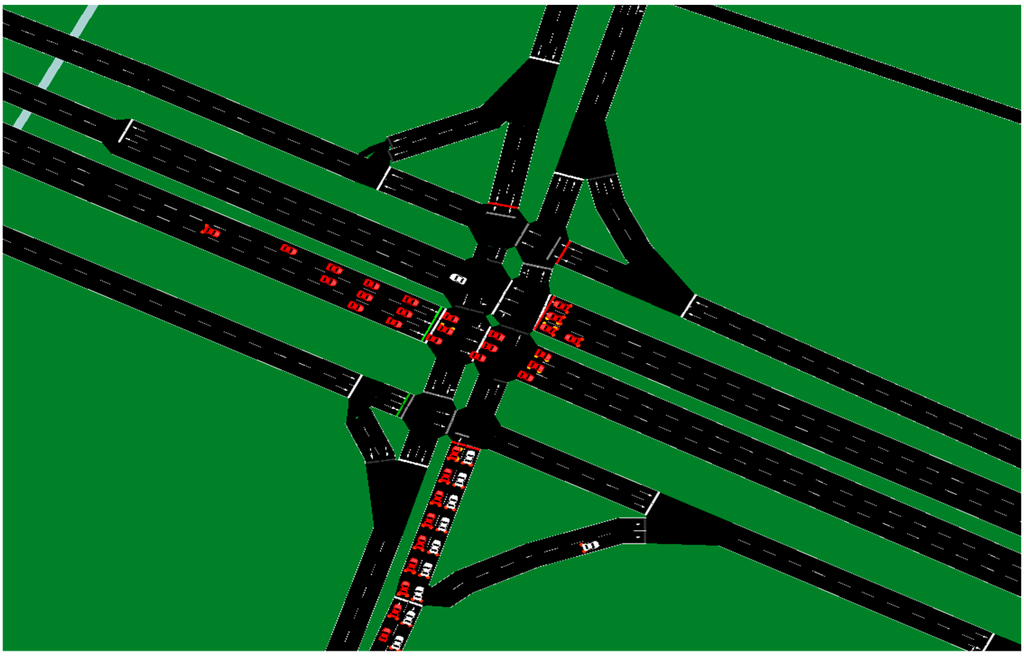
\includegraphics{sumo-simulator}
	\caption{Ejemplo de pantalla del simulador \gls{sumo}. Además de entorno de simulación propiamente dicho, \gls{sumo} provee de una interfaz gráfica que permite una visualización general, de zonas y de elementos en concreto a la vez que permite la variación de configuración de la simulación durante el desarrollo de la misma.}
	\label{fig:sumo-simulator}
\end{figure}

\begin{itemize}
	\item Multimodalidad permitiendo modelar no sólo tráfico de vehículos sino de peatones, bicicletas, trenes e incluso de barcos.
	\item Vehículos de diferentes tipologías, Simulación con y sin colisiones de vehículos.
	\item Diferentes tipos de vehículos y de carreteras, cada una con diferentes carriles y éstas con diferentes subdivisiones de subcarriles (diseño conceptual para permitir las simulaciones )
\end{itemize}

Al estar licenciado bajo la licencia \gls{gpl}, su distribución implica a su vez la distribución de su código fuente. Esto permite la modeificación de su comportamiento y el desarrollo de nuevos modelos integrados dentro del simulador. Sin embargo nosotros no haremos uso de esta característica, sino que usaremos \gls{sumo} como aplicación servidor y el módulo \gls{traci} como aplicación cliente desde donde gestionar todos los aspectos de cada simulación.

\subsection{La interfaz \glsentrylong{traci}}